
\section{Test und Messung von Kennwerten der Asynchronmaschine}

Am Ende der Inbetriebnahme haben wir verschieden Tests und Messungen gemacht. 
Unter anderem wurden die Ansteuersignale zweier Schalter aufgezeichnet. Man sieht gut, dass sich der Duty Cycle sinuidal verändert und es lange Aus-Zeiten gibt(ein hoher Pegel öffnet den Schalter). Die Phasenverschiebung der beiden Sinui beträgt 120 Grad, was sich aus dem Bild näherungsweise ermitteln lässt.
\begin{figure}[H]
		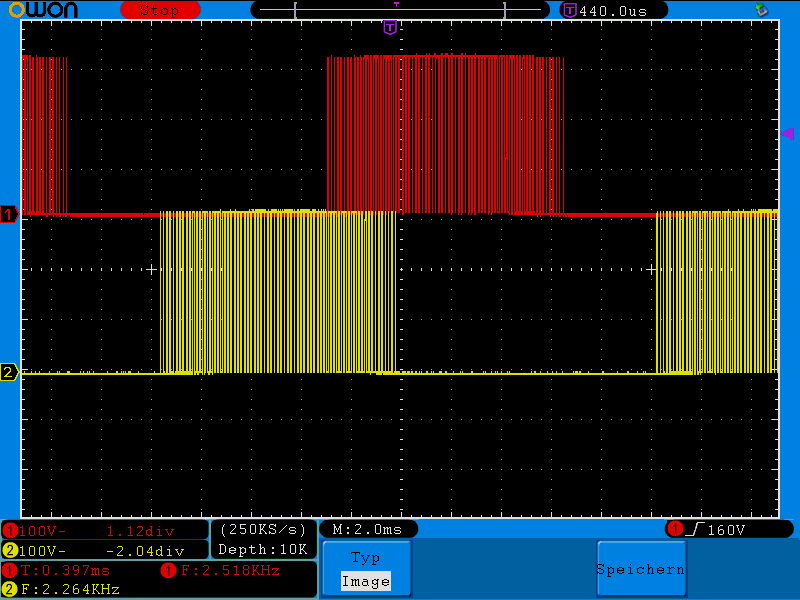
\includegraphics[width=0.5\textwidth]{uwgeregelt.png}
		\caption{Schaltmomente)}
		\label{fig:rreibChart}
	\end{figure}
	Des Weiteren wurde der Strom durch eine Phase im Leerlauf mit einer Stromzange ermittelt. Leerlauf heißt, dass die Anschlüsse des Generators offen waren. Hierbei gilt, dass 100mV einem A entsprechen. Zu sehen sind neben mehreren Messfehlern vor allem die Sinuskurvenform des Stroms. Aufgrund des Messaufbaus war es leider nicht möglich Spannung und Strom zum selben Zeitpunkt zu messen, wir würden dabei eine Phasenverschiebung auf Grund der Induktivität der Motorinduktivität erwarten.  
	\begin{figure}[H]
		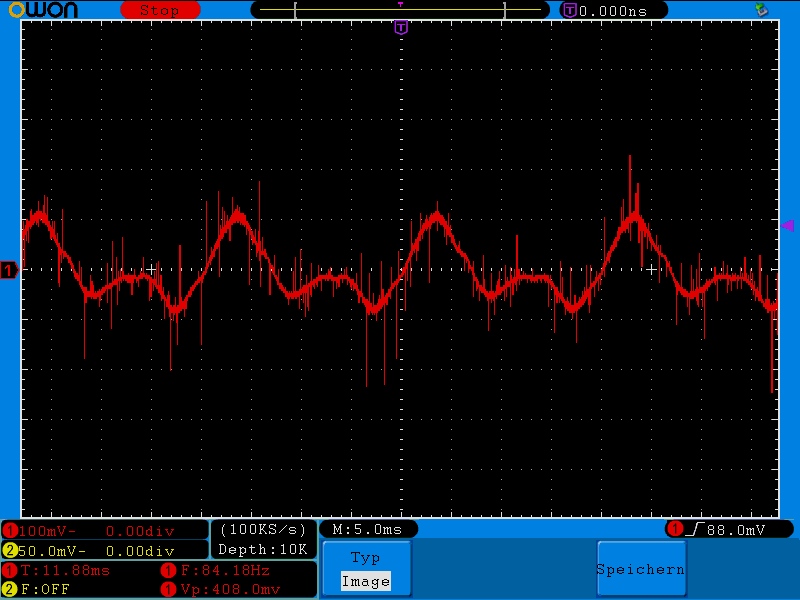
\includegraphics[width=0.5\textwidth]{strom1Phase.png}
		\caption{Strommmessung einer Phase}
		\label{fig:rreibChart}
	\end{figure}